\begin{enumerate}
 \item L'inégalité demandée résulte de l'inégalité des accroissements finis appliquée à la fonction $t\rightarrow \ln t$ entre $x$ et $x+1$. En effet la dérivée est $\frac{1}{t}$ qui est supérieur ou égal à $\frac{1}{1+t}$ dans l'intervalle considéré.
 \item Notons $\varphi$ la fonction à étudier. \'Ecrivons la sous forme exponentielle avant de la dériver.
\begin{displaymath}
 \varphi(x) = 
e^{x\left(\ln(x+1)-\ln x \right) }>0
\end{displaymath}
\begin{multline*}
 \varphi'(x)=\left(\ln(x+1)-\ln(x)+\frac{x}{x+1}-1 \right)\varphi(x)\\
 =\left(\ln(x+1)-\ln(x)-\frac{x}{x+1} \right)\varphi(x)\geq 0
\end{multline*}
d'après l'inégalité de la première question. La fonction $\varphi$ est donc croissante.
\begin{figure}[h!]
 \centering
 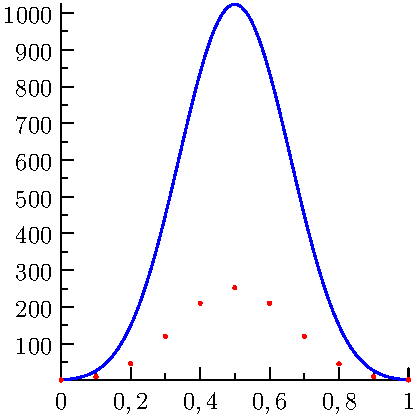
\includegraphics{Cmajcobi_1.pdf}
 % Cmajcobi_1.pdf: 0x0 pixel, 0dpi, 0.00x0.00 cm, bb=
 \caption{Coefficient du binôme et fonction $e^{nH}$ pour $n=10$.}
 \label{fig:Cmajcobi_1}
\end{figure}
 \item Fixons un entier $n$ et notons $I_k$ l'inégalité à démontrer:
\begin{displaymath}
 (I_k)\hspace{1cm}\binom{n}{k}\leq\frac{n^n}{k^k(n-k)^{n-k}}
\end{displaymath}
Remarquons d'abord que $I_0$ est vérifiée car elle revient à $1\leq 1$. Remarquons ensuite que les deux expressions à comparer sont conservées par le changement $k\rightarrow n-k$. Il suffit donc de montrer $I_k$ pour les $k$ tels que $k<n-k$.\newline
On va montrer que $I_k\Rightarrow I_{k+1}$ pour $k<n-k$.\newline
Supposons $I_k$ et considérons le coefficient du binôme suivant:
\begin{displaymath}
 \binom{n}{k+1}=\frac{n(n-1)\cdots(n-k)}{(k+1)!}=\frac{n-k}{k+1}\binom{n}{k}\\
\leq \frac{n^n}{(k+1)k^k(n-k)^{n-(k+1)}}
\end{displaymath}
 d'après $I_k$. Il suffit donc de montrer:
\begin{displaymath}
 \frac{n^n}{(k+1)k^k(n-k)^{n-(k+1)}}
\leq \frac{n^n}{(k+1)^{k+1}(n-k-1)^{n-k-1}}
\end{displaymath}
ou encore $x_k\leq 1$ avec 
\begin{multline*}
 x_k = \frac{n^n}{(k+1)k^k(n-k)^{n-(k+1)}} \frac{(k+1)^{k+1}(n-k-1)^{n-k-1}}{n^n}\\
=\left(\frac{k+1}{k} \right)^k\left(\frac{n-k}{n-k-1} \right)^{-(n-k-1)}
= \frac{\varphi(k)}{\varphi(n-k-1)}  
\end{multline*}
avec la fonction $\varphi$ de la deuxième question. Comme $\varphi$ est croissante et $k\leq n-k-1$, on a bien $\varphi(k)\leq \varphi(n-k-1)$ ce qui achève la démonstration.

Cette démonstration est bien laborieuse à côté de celle ci trouvée par un étudiant\footnote{Thomas Lehéricy}:\newline
Il s'agit en fait de démontrer que
\begin{displaymath}
 \binom{n}{k}k^k(n-k)^{n-k}\leq n^n
\end{displaymath}
Sous cette forme, le membre de gauche apparait clairement comme un terme (celui pour lequel $i=k$) dans une formule du binôme
\begin{displaymath}
 \binom{n}{k}k^k(n-k)^{n-k} \leq \sum_{i=0}^n \binom{n}{i}k^i(n-k)^{n-i}=(k+(n-k))^n=n^n
\end{displaymath}

 \item  L'inégalité de la question précédente s'exprime avec $H$ et l'exponentielle car
\begin{displaymath}
 \frac{n^n}{k^k(n-k)^{n-k}} =\left( \frac{n}{k}\right)^k \left( \frac{n}{n-k}\right)^{(n-k)}
=e^{-\left(k\ln(\frac{k}{n})+ (n-k)\ln(\frac{n-k}{n})\right) } 
=e^{nH(\frac{k}{n})}
\end{displaymath}
La figure \ref{fig:Cmajcobi_1} montre que cette inégalité est très imprécise pour les coefficients du milieu.
\end{enumerate}
